\subsection{KPI Forecasting Results}
\label{sec:forecasting_results}
\label{sec:results}

Continuous KPI forecasting performance across horizons is reported in Table~\ref{tab:forecasting_main}, with the main CET-STGL, classical and event-based trends visualized in Fig.~\ref{fig:forecasting}. CET-STGL-sklearn is competitive with the feature-engineered Ridge baseline on the primary-KPI subset. At $h=1$\,h, CET-STGL-sklearn obtains MAE/RMSE values of 2.183/4.635, compared with 2.219/4.698 for Ridge/Logistic. At $h=3$\,h and $h=6$\,h, CET-STGL-sklearn remains lower in MAE than Ridge/Logistic. At $h=12$\,h, the two models are close: CET-STGL-sklearn has slightly lower MAE, while Ridge/Logistic has slightly lower RMSE.

The no-alarm CET-STGL ablation achieves lower MAE and RMSE than the full CET-STGL instantiation at all four horizons. The pattern is consistent with the high sparsity of alarm observations: active alarms appear in only 1.62\% of rows, while routine KPI variation is largely described by continuous temporal and cell-specific patterns. From a reliability perspective, the ablation indicates that sparse alarms should be treated as contextual evidence rather than universal predictors of routine KPI evolution. Standalone event-intensity baselines remain weak for continuous forecasting, with Hawkes-only producing an $h=1$\,h MAE/RMSE of 4.578/7.981. The fixed LSTM baseline has higher primary-KPI MAE/RMSE than CET-STGL-sklearn and Ridge/Logistic at all horizons, and the fixed TCN baseline is weaker under the same protocol.

\begin{table}[t]
\centering
\caption{Primary-KPI forecasting summary for runnable models.}
\label{tab:forecasting_main}
\scriptsize
\setlength{\tabcolsep}{4pt}
\begin{tabular}{llrrr}
\toprule
Model & H & MAE & RMSE & MAPE \\
\midrule
CET-STGL without alarm tokens & 1 & 2.157 & 4.602 & 42.411 \\
CET-STGL-sklearn & 1 & 2.183 & 4.635 & 42.642 \\
Event-attention-only & 1 & 4.630 & 8.276 & 82.519 \\
Hawkes-only & 1 & 4.578 & 7.981 & 82.261 \\
LSTM & 1 & 3.774 & 6.606 & 68.954 \\
TCN & 1 & 13.360 & 51.673 & 131.255 \\
Ridge/Logistic & 1 & 2.219 & 4.698 & 43.599 \\
Ridge/Logistic without alarms & 1 & 2.203 & 4.671 & 43.382 \\
CET-STGL without alarm tokens & 3 & 2.490 & 4.974 & 46.807 \\
CET-STGL-sklearn & 3 & 2.537 & 5.083 & 47.162 \\
Event-attention-only & 3 & 4.635 & 8.326 & 82.776 \\
Hawkes-only & 3 & 4.581 & 8.038 & 82.515 \\
LSTM & 3 & 3.822 & 6.907 & 72.139 \\
TCN & 3 & 6.580 & 16.235 & 116.662 \\
Ridge/Logistic & 3 & 3.071 & 5.684 & 56.382 \\
Ridge/Logistic without alarms & 3 & 3.036 & 5.586 & 56.015 \\
CET-STGL without alarm tokens & 6 & 3.145 & 5.605 & 56.843 \\
CET-STGL-sklearn & 6 & 3.197 & 5.853 & 57.264 \\
Event-attention-only & 6 & 4.629 & 8.277 & 83.117 \\
Hawkes-only & 6 & 4.578 & 7.873 & 82.871 \\
LSTM & 6 & 3.991 & 7.053 & 73.741 \\
TCN & 6 & 7.660 & 19.911 & 121.740 \\
Ridge/Logistic & 6 & 3.338 & 5.940 & 61.590 \\
Ridge/Logistic without alarms & 6 & 3.318 & 5.884 & 61.272 \\
CET-STGL without alarm tokens & 12 & 2.515 & 5.051 & 47.283 \\
CET-STGL-sklearn & 12 & 2.604 & 5.442 & 47.682 \\
Event-attention-only & 12 & 4.671 & 8.622 & 83.341 \\
Hawkes-only & 12 & 4.572 & 7.888 & 83.061 \\
LSTM & 12 & 3.892 & 7.066 & 73.416 \\
TCN & 12 & 11.522 & 41.975 & 124.861 \\
Ridge/Logistic & 12 & 2.640 & 5.391 & 49.140 \\
Ridge/Logistic without alarms & 12 & 2.593 & 5.135 & 48.806 \\
\bottomrule
\end{tabular}

\end{table}


\subsection{Weak Degradation Classification Results}
\label{sec:classification_results}

Weak degradation classification performance is summarized in Table~\ref{tab:classification_main}, while Fig.~\ref{fig:classification} gives the corresponding CET-STGL, classical and event-based comparisons. At $h=1$\,h, CET-STGL-sklearn obtains an AUPRC of 0.466 and F1-score of 0.479, performing comparably to the feature-engineered linear logistic baselines (AUPRC 0.471--0.476). Across longer horizons, AUPRC values among the feature-engineered baselines remain relatively close, whereas threshold-dependent F1, Precision and Recall vary substantially across models and horizons. LSTM provides a useful neural sequence comparator and is competitive on AUPRC at some horizons, but it does not dominate the linear and CET-STGL variants across metrics.

Event-only models exhibit limited discriminative power for threshold-based degradation prediction, with Hawkes-only and Event-attention-only attaining lower AUPRC scores of 0.247 and 0.257 at $h=1$\,h, respectively. Sparse network alarms are weak standalone predictors under the present protocol.

\begin{table}[t]
\centering
\caption{Weak KPI degradation classification summary.}
\label{tab:classification_main}
\scriptsize
\setlength{\tabcolsep}{4pt}
\begin{tabular}{llrrrr}
\toprule
Model & H & AUPRC & F1 & Prec. & Recall \\
\midrule
CET-STGL without alarm tokens & 1 & 0.470 & 0.361 & 0.221 & 0.975 \\
CET-STGL-sklearn & 1 & 0.466 & 0.479 & 0.395 & 0.608 \\
Event-attention-only & 1 & 0.257 & 0.331 & 0.226 & 0.620 \\
Hawkes-only & 1 & 0.247 & 0.327 & 0.218 & 0.656 \\
LSTM & 1 & 0.448 & 0.404 & 0.277 & 0.748 \\
TCN & 1 & 0.270 & 0.389 & 0.277 & 0.652 \\
Ridge/Logistic & 1 & 0.471 & 0.477 & 0.418 & 0.556 \\
Ridge/Logistic without alarms & 1 & 0.476 & 0.480 & 0.396 & 0.610 \\
CET-STGL without alarm tokens & 3 & 0.399 & 0.348 & 0.520 & 0.262 \\
CET-STGL-sklearn & 3 & 0.375 & 0.147 & 0.570 & 0.084 \\
Event-attention-only & 3 & 0.249 & 0.331 & 0.218 & 0.684 \\
Hawkes-only & 3 & 0.233 & 0.326 & 0.218 & 0.649 \\
LSTM & 3 & 0.370 & 0.390 & 0.268 & 0.717 \\
TCN & 3 & 0.220 & 0.334 & 0.226 & 0.640 \\
Ridge/Logistic & 3 & 0.341 & 0.320 & 0.191 & 0.996 \\
Ridge/Logistic without alarms & 3 & 0.336 & 0.212 & 0.445 & 0.139 \\
CET-STGL without alarm tokens & 6 & 0.334 & 0.331 & 0.200 & 0.975 \\
CET-STGL-sklearn & 6 & 0.318 & 0.389 & 0.284 & 0.618 \\
Event-attention-only & 6 & 0.215 & 0.352 & 0.245 & 0.623 \\
Hawkes-only & 6 & 0.294 & 0.318 & 0.215 & 0.611 \\
LSTM & 6 & 0.350 & 0.368 & 0.246 & 0.727 \\
TCN & 6 & 0.199 & 0.313 & 0.211 & 0.605 \\
Ridge/Logistic & 6 & 0.309 & 0.315 & 0.402 & 0.259 \\
Ridge/Logistic without alarms & 6 & 0.284 & 0.363 & 0.245 & 0.698 \\
CET-STGL without alarm tokens & 12 & 0.377 & 0.334 & 0.201 & 0.989 \\
CET-STGL-sklearn & 12 & 0.373 & 0.324 & 0.193 & 0.997 \\
Event-attention-only & 12 & 0.240 & 0.340 & 0.238 & 0.590 \\
Hawkes-only & 12 & 0.247 & 0.322 & 0.219 & 0.608 \\
LSTM & 12 & 0.380 & 0.376 & 0.262 & 0.666 \\
TCN & 12 & 0.190 & 0.289 & 0.196 & 0.548 \\
Ridge/Logistic & 12 & 0.381 & 0.334 & 0.201 & 0.983 \\
Ridge/Logistic without alarms & 12 & 0.396 & 0.335 & 0.202 & 0.983 \\
\bottomrule
\end{tabular}

\end{table}


\subsection{Weak Alarm-Candidate Prioritization Results}
\label{sec:ranking_results}

Weak alarm-candidate ranking consistency is evaluated in Table~\ref{tab:ranking_main} and Fig.~\ref{fig:ranking}. Both the target candidate and the ranking score are derived from association-based weak rules using event intensity and train-only lift. Values of 1.000 therefore indicate agreement with the weak protocol, not verified operational fault localization. The Hawkes-only and no-dynamic-graph rows act as diagnostic checks because they retain event recency but remove the full association-derived scoring structure, yielding $\mathrm{Hit}(1)$ values near 0.80 and MRR values near 0.89.

\begin{table}[t]
\centering
\caption{Weak root-cause candidate ranking summary.}
\label{tab:ranking_main}
\scriptsize
\setlength{\tabcolsep}{4pt}
\begin{tabular}{llrrrr}
\toprule
Model & H & N & Hit@1 & MRR & nDCG@5 \\
\midrule
CET w/o dynamic event graph & 1 & 2682 & 0.808 & 0.895 & 0.920 \\
CET-STGL-sklearn & 1 & 2682 & 1.000 & 1.000 & 1.000 \\
Event-attention-only & 1 & 611 & 1.000 & 1.000 & 1.000 \\
Hawkes-only & 1 & 2682 & 0.808 & 0.895 & 0.920 \\
Ridge/Logistic & 1 & 611 & 0.930 & 0.960 & 0.971 \\
CET w/o dynamic event graph & 3 & 2671 & 0.807 & 0.894 & 0.919 \\
CET-STGL-sklearn & 3 & 2671 & 1.000 & 1.000 & 1.000 \\
Event-attention-only & 3 & 609 & 1.000 & 1.000 & 1.000 \\
Hawkes-only & 3 & 2671 & 0.807 & 0.894 & 0.919 \\
Ridge/Logistic & 3 & 609 & 0.923 & 0.958 & 0.969 \\
CET w/o dynamic event graph & 6 & 2645 & 0.805 & 0.893 & 0.918 \\
CET-STGL-sklearn & 6 & 2645 & 1.000 & 1.000 & 1.000 \\
Event-attention-only & 6 & 614 & 1.000 & 1.000 & 1.000 \\
Hawkes-only & 6 & 2645 & 0.805 & 0.893 & 0.918 \\
Ridge/Logistic & 6 & 614 & 0.917 & 0.955 & 0.967 \\
CET w/o dynamic event graph & 12 & 2617 & 0.804 & 0.892 & 0.918 \\
CET-STGL-sklearn & 12 & 2617 & 1.000 & 1.000 & 1.000 \\
Event-attention-only & 12 & 649 & 1.000 & 1.000 & 1.000 \\
Hawkes-only & 12 & 2617 & 0.804 & 0.892 & 0.918 \\
Ridge/Logistic & 12 & 649 & 0.928 & 0.962 & 0.972 \\
\bottomrule
\end{tabular}

\vspace{0.3em}
\footnotesize{Note. Ranking uses weak alarm-lift/event-intensity proxy labels, not expert-confirmed root-cause localization. Perfect scores indicate proxy consistency when scoring overlaps with weak-label construction. Neural baselines are not run because PyTorch is unavailable. The event graph is causal-inspired / causal discovery-based, not confirmed causality.}
\end{table}


\subsection{Ablation and Component Analysis}
\label{sec:ablation_results}

Ablation deltas relative to the full CET-STGL instantiation are reported in Table~\ref{tab:ablation_main} and Fig.~\ref{fig:ablation}. Removing alarm tokens lowers average forecasting MAE in the reported primary-KPI summary. In the evaluated slice, alarm and graph features do not improve aggregate forecasting consistently, although alarm information remains relevant to the weak association-based prioritization protocol. The ablation evidence therefore supports the methodological separation between continuous KPI dynamics, sparse event context and association-based prioritization.

Component-wise ablations highlight the contribution of specific structural choices:
\begin{enumerate}
    \item \textbf{Patch features:} Removing tokenization increases average forecasting MAE, supporting the use of local level and slope summaries for KPI histories.
    \item \textbf{Dynamic event graph:} Removing the dynamic event graph reduces consistency with the association-derived ranking rule, as expected. The result reflects protocol consistency rather than independent validation of operational fault-localization utility.
\end{enumerate}

\begin{table}[t]
\centering
\caption{Ablation deltas averaged over horizons relative to CET-STGL-sklearn.}
\label{tab:ablation_main}
\tiny
\setlength{\tabcolsep}{2pt}
\begin{tabular}{llrrr}
\toprule
Ablation row & Removed component & $\Delta$ MAE & $\Delta$ AUPRC & $\Delta$ MRR \\
\midrule
CET-STGL without alarm tokens & no\_alarm & -0.054 & 0.012 &  \\
CET-STGL without cross-cell graph & no\_cross\_cell\_graph & -0.003 & -0.000 & 0.000 \\
CET-STGL without dynamic event graph & no\_dynamic\_graph & 0.000 & 0.001 & -0.107 \\
CET-STGL without Hawkes intensity & no\_hawkes\_intensity & 0.000 & 0.001 & 0.000 \\
CET-STGL without tokenization & no\_tokenization & 0.200 & -0.017 & 0.000 \\
\bottomrule
\end{tabular}

\end{table}


\begin{figure}[t]
    \centering
    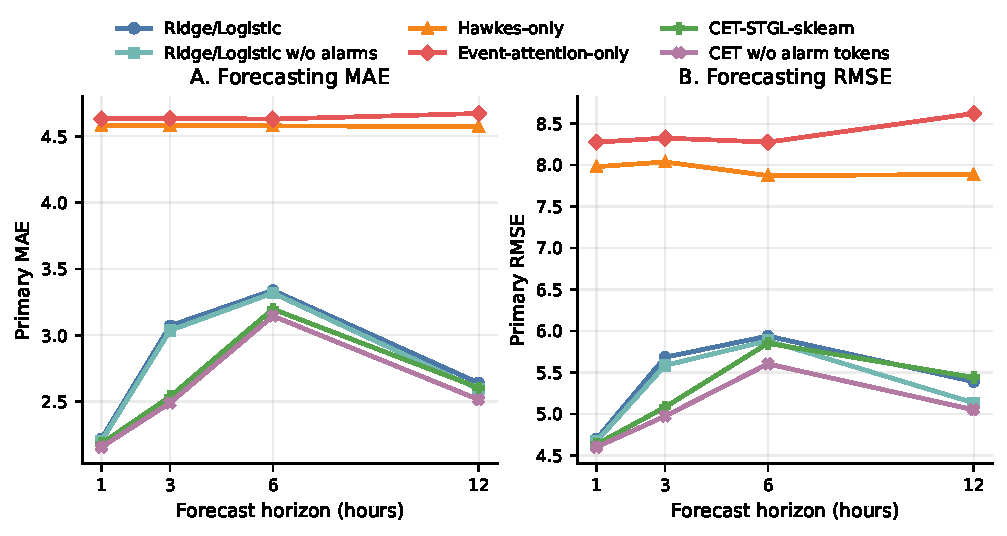
\includegraphics[width=\linewidth]{figures/Fig1_forecasting_vs_horizon.pdf}
    \caption{Primary-KPI forecasting error versus prediction horizon.}
    \label{fig:forecasting}
\end{figure}

\begin{figure}[t]
    \centering
    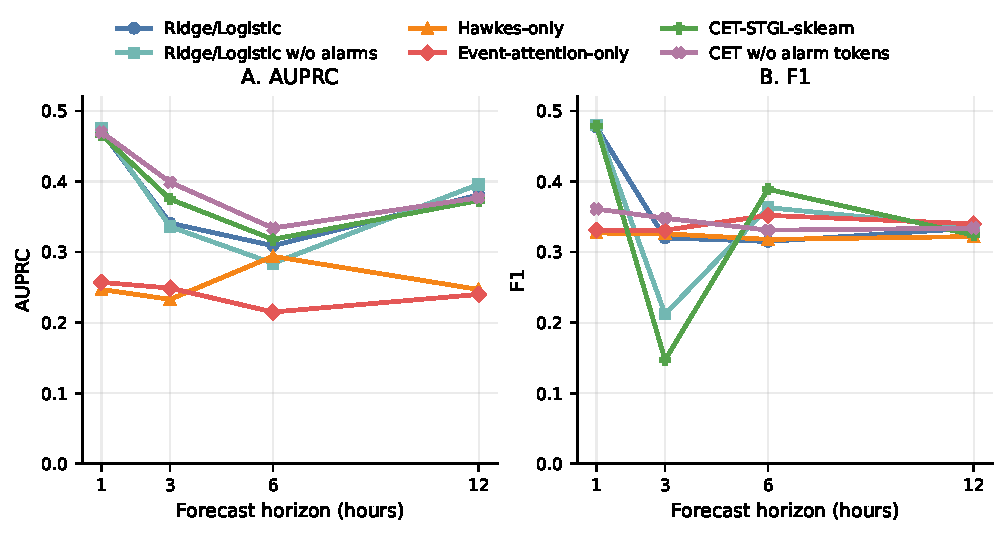
\includegraphics[width=\linewidth]{figures/Fig2_classification_comparison.pdf}
    \caption{KPI degradation classification performance versus prediction horizon.}
    \label{fig:classification}
\end{figure}

\begin{figure}[t]
    \centering
    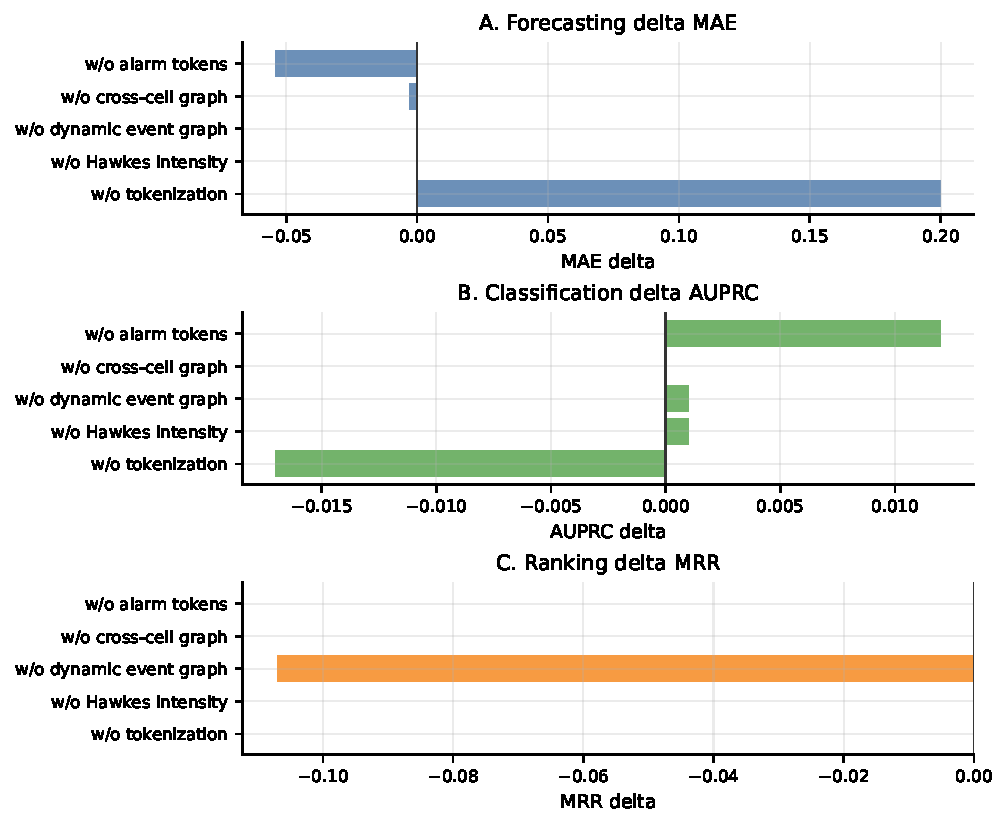
\includegraphics[width=\linewidth]{figures/Fig3_ablation_delta.pdf}
    \caption{Ablation deltas relative to CET-STGL-sklearn.}
    \label{fig:ablation}
\end{figure}

\begin{figure}[t]
    \centering
    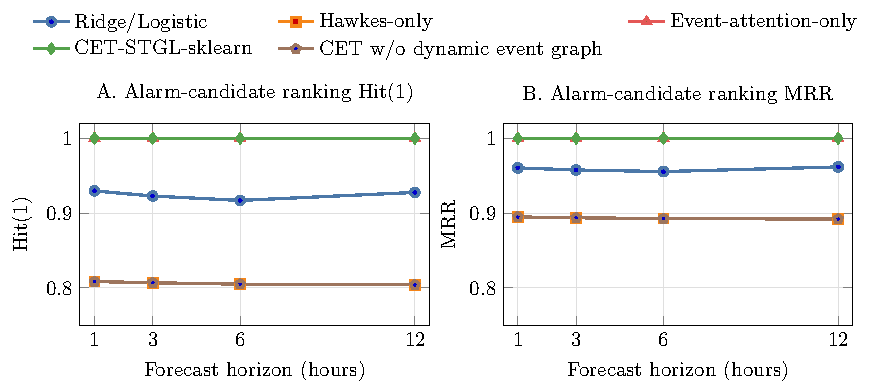
\includegraphics[width=\linewidth]{figures/Fig4_weak_ranking_comparison.pdf}
    \caption{Weak alarm-candidate ranking consistency versus prediction horizon.}
    \label{fig:ranking}
\end{figure}
